\documentclass{article}

\usepackage{ulem,xcolor,fixltx2e}
\usepackage[a4paper]{geometry}
\geometry{left=1cm,right=1cm,top=1cm,bottom=1.5cm}

\usepackage{xecjk}
\setCJKmainfont{Microsoft YaHei} % Set default chinese... font

\usepackage{listings}

\usepackage[unicode=true]{hyperref}
\urlstyle{same} % Don't use monospace font for urls

\usepackage{graphicx,grffile}
\graphicspath{.} % Set path
\makeatletter
\def\maxwidth{\ifdim\Gin@nat@width>\linewidth\linewidth\else\Gin@nat@width\fi}
\def\maxheight{\ifdim\Gin@nat@height>\textheight\textheight\else\Gin@nat@height\fi}
\makeatother
% Scale images if necessary, so that they will not overflow the page
% margins by default, and it is still possible to overwrite the defaults
% using explicit options in \includegraphics[width, height, ...]{}
\setkeys{Gin}{width=\maxwidth,height=\maxheight,keepaspectratio}

\makeatletter
\def\UrlAlphabet{
      \do\a\do\b\do\c\do\d\do\e\do\f\do\g\do\h\do\i\do\j
      \do\k\do\l\do\m\do\n\do\o\do\p\do\q\do\r\do\s\do\t
      \do\u\do\v\do\w\do\x\do\y\do\z\do\A\do\B\do\C\do\D
      \do\E\do\F\do\G\do\H\do\I\do\J\do\K\do\L\do\M\do\N
      \do\O\do\P\do\Q\do\R\do\S\do\T\do\U\do\V\do\W\do\X
      \do\Y\do\Z}
\def\UrlDigits{\do\1\do\2\do\3\do\4\do\5\do\6\do\7\do\8\do\9\do\0}
\g@addto@macro{\UrlBreaks}{\UrlOrds}
\g@addto@macro{\UrlBreaks}{\UrlAlphabet}
\g@addto@macro{\UrlBreaks}{\UrlDigits}
\makeatother % Url break

\setlength{\emergencystretch}{3em}  % Prevent overfull lines

\linespread{1.5}

\renewcommand{\CJKglue}{\hskip 2pt}

\lstset{
  keywordstyle=\color{blue!70},
  commentstyle=\color{red!50!green!50!blue!50},
  rulesepcolor=\color{red!20!green!20!blue!20},
  language=c++
}

\begin{document}

\title{ \bf 课程表助手 }
\author{}
\date{2019}
\maketitle

\tableofcontents

\pagebreak

\section{项目简介}

由于高职院校普遍存在教室资源和教师数量不足的问题,导致教师的课程安排比较杂乱,没有规
律,学生也经常因此而忘记去上课,由此经常造成教学事故的发生。为有效避免教学事故的发生,
我们团队预备设计一个基于 Android 平台的课表提醒实用 APP 程序。

未来的时代必定是个更加信息化的时代,手机正成为我们生活必不可少的部分,针对日常快节奏的
生活方式,许多手机应用软件应运而生,潜移默化的改变了人们的生活,同时,网上交易也日渐成为
一种常见的交易方式。利用手机解决各种学生活上的烦恼,已成为一种社会潮流和风尚。我们根
据实际生活遇到的问题,并提出了这样的想法。我们这款产品的主要对象是大学生,大学生普遍都
有网上搜索和购物的经历,因此他们对这款软件不会觉得陌生,而且更加熟悉它的操作流程,而且
这款软件是以解决学生迫切的学习生活问题为出发点的。我们的核心竞争力是立足于学生,服务
于学生,更容易取得学生的共鸣

\section{功能设想}

这个APP程序计划包含课程表导入模块、定时提醒模块。程序将教师课表导入后,自动提取课表
的上课日期、上课时间、上课地点和任课课程,在上课前 20 分钟给任课教师的手机发送上课提
醒信息,提醒内容包括上课时间、地点和课程名称等,实现了对教师的课前即时提醒。这个程序
还考虑到了课程表中课程安排的某些特殊性,如开学日期设置等,可以满足任课教师和学生的特
定需求。

\section{功能实现}

  \subsection{技术选型}

    由于项目目的为学习与应用,故采用了跨平台框架\href{https://flutter.dev/}{flutter},兼顾iOS平台,而非单纯的\textit{java}、
    \textit{kotlin}、\textit{objective-c}或\textit{swift}。

  \subsection{开学日期设置}

    \bf 暂未实现

  \subsection{课程导入}

    \bf 暂未实现

  \subsection{课程创建}

    点击 + 图标进入 \uline{添加课程} 界面新建课程。支持修改课程名称、教室、教师、星
    期、周数和上课时间段。对于时间段可能交叉的课程,时间段相同的可重叠,否则不能添加。

  \subsection{课程修改}

    点击已经存在的课程,根据当前时间段节数:
    \begin{itemize}
      \item 只有一节。 直接进入 \uline{修改课程} 界面。
      \item 有多节。 显示当前课程列表,选中相应课程后进入 \uline{修改课程} 界面。
    \end{itemize}

  \subsection{定时提醒}

    \subsubsection{时间设置}

      点击课程列表左列数字,可设置相应课时的铃声提醒时间。

    \subsubsection{提醒}

      到设置时间出现提醒界面(时间、地点和课程名称等)并响铃

    \subsubsection{*铃声设置}

      进入设置界面可设置提醒铃声

  \subsection{周数选择}

    点击主界面上方周数后,可设置当前所在周数

  \subsection{*主题设置}

    进入设置界面可设置界面主题

\section{界面}

  \subsection{主界面}

    月份与星期在同一行。考虑到由于时间段问题,课程会有跨行行为,为便于实现,课程显示部分均采用列布局。

  \subsection{课程创建}

    输入和选择项都置于\uline{ExpansionTile},用于选择性展开,节省空间。取消按钮使用浅色扁平类型,
    确认按钮使用突出类型,以符合正常使用中的用户视觉交互。

  \subsection{课程修改}

    复用课程创建界面,删除按钮改为红色,起警示作用。

    \begin{figure}[ht]
      \begin{minipage}[h]{0.4\linewidth}
        \centering
        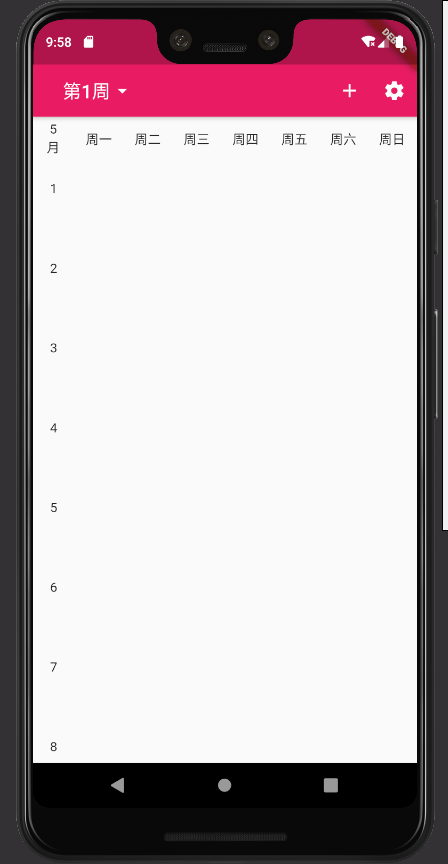
\includegraphics[height=\linewidth]{main.png}
        \caption{主界面}
        \label{fig:main}
      \end{minipage}
      \hfill
      \begin{minipage}[h]{0.4\linewidth}
        \centering
        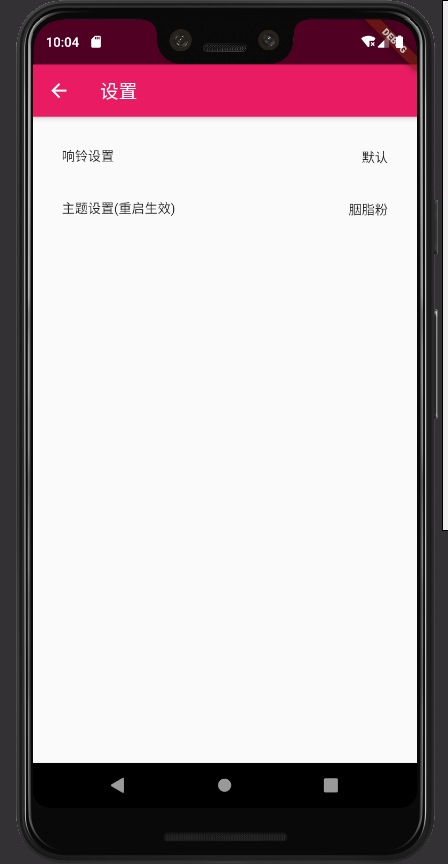
\includegraphics[height=\linewidth]{settings.png}
        \caption{设置}
        \label{fig:settings}
      \end{minipage}
    \end{figure}

    \begin{figure}[ht]
      \begin{minipage}[h]{0.4\linewidth}
        \centering
        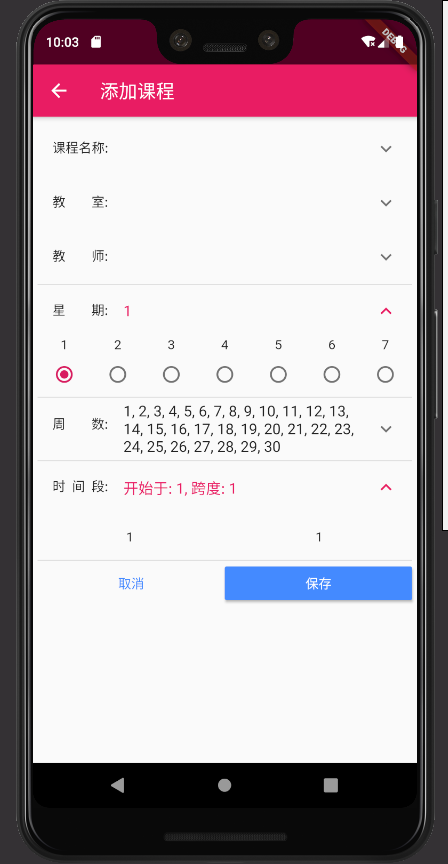
\includegraphics[height=\linewidth]{create.png}
        \caption{添加课程}
        \label{fig:create}
      \end{minipage}
      \hfill
      \begin{minipage}[h]{0.4\linewidth}
        \centering
        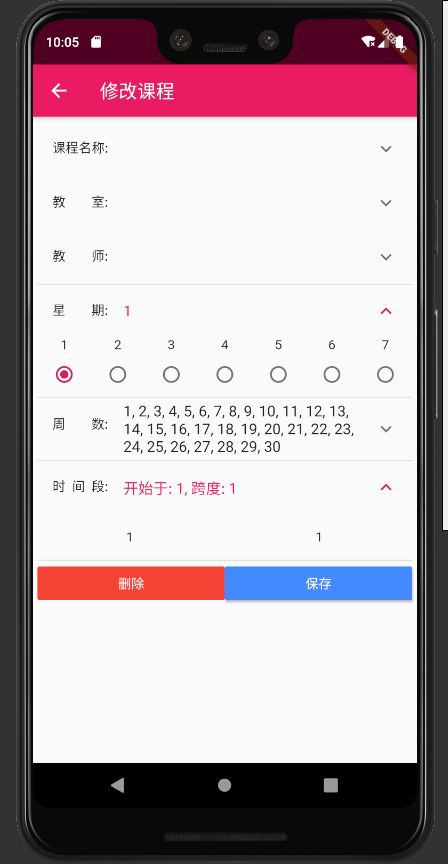
\includegraphics[height=\linewidth]{modify.png}
        \caption{修改课程}
        \label{fig:modify}
      \end{minipage} 
    \end{figure}

\section{过程中的问题与解决方案}

  \subsection{已解决的问题}

    \begin{enumerate}
      \item 布局溢出\textsuperscript{\cite{ref:overflow}}。布局时,子组件可能会由于大小问题溢出父组件/设备屏幕。这种情况在子组件有
      固定宽/高时最明显。

        \textbf{方案分析:}一般在溢出的组件外包装一层 \uline{Expanded}\textsuperscript{\cite{ref:Expanded}} 或 \uline{Container}\textsuperscript{\cite{ref:Container}} 。

      \item 课程交叉检测。添加课程时,可能与已有课程时间段相交。

        \textbf{方案分析:}需检测课程起始时间段与所跨行数。

        \begin{lstlisting}[frame=shadowbox]
          ...
          // 返回是否相交且未重叠
          return list.any((course) {
            // 检查是否相交
            if ((start + step > course.start) &&
                (start < course.start + course.step)) {
              // 检查是否重叠
              if ((start == course.start) && (step == course.step)) {
                return false;
              } else {
                return true;
              }
            }
            return false;
          });
        \end{lstlisting}

      \item 课程重叠。

        \textbf{方案分析:}将重叠课程置于\uline{Stack}\textsuperscript{\cite{ref:Stack}}组件直接重叠,同时下方显示当前组的课程数

      \item 课程布局。因存在无课程的空白空间,不能在一列直接放置课程。

        \textbf{方案分析:}非绝对定位方案:在课程前添加足够高的空白块,撑起布局。

        \begin{lstlisting}[frame=shadowbox]
          // 课程列表填充空白块
          List getFilledCourses({
            // 课程列表
            @required List<CourseModel> courses,
            ...
          }) {
            if (courses.length == 0) return [];
            // 最终返回的列表
            List ret = [];
            int prevStart = 0;
            int prevStep = 1;
            ...
            courses.forEach((course) {
              // 判断两个课程间是否有空白
              if (course.start > (prevStart + prevStep)) {
                // 两个课程间有空白则填充空白块
                ret.add(EmptyModel(
                  minHeight: minHeight,
                  weekday: weekday,
                  start: prevStart + prevStep,
                  step: course.start - (prevStart + prevStep),
                ));
                prevStart = prevStart + prevStep - (prevStart + prevStep);
                prevStep = course.start + course.step;
              } else {
                prevStart = course.start;
                prevStep = course.step;
              }
              ret.add(course);
            });
            // 如果最后有空白,也填充空白块
            if (prevStart + prevStep - 1 < getRowCount()) {
              ret.add(EmptyModel(
                minHeight: minHeight,
                weekday: weekday,
                start: prevStart + prevStep,
                step: getRowCount() - (prevStart + prevStep) + 1,
              ));
            }
            return ret;
          }
        \end{lstlisting}
    \end{enumerate}

  \subsection{未解决的问题}

    \begin{enumerate}
      \item 不能导入课程。

        \textbf{可能方案分析:}无。

      \item 不能设置开学日期。

        \textbf{可能方案分析:}设置第一周,以第一周为准依次累加。

      \item 周数不能随时间变化。

        \textbf{可能方案分析:}获取开学周,依次累加。

      \item 点击课程列表中某课程,修改后保存返回,列表不更新。

        \textbf{可能方案分析:}无。

      \item 一切取消设置时间的操作(点击 \textit{cancel} 或 空白处)都会使当前已设置时间清除。

        \textbf{可能方案分析:}由于取消设置时程序会抛出异常,在捕获异常时根据抛出的异常类型判断
        \textit{cancel / dismiss}。

      \item 定时提醒在熄屏后失效。

        \textbf{可能方案分析:}当前使用 \textit{dart:async}\textsuperscript{\cite{ref:async}} 中
        的 \textit{Future.delayed()},设备熄屏后可能进入低功耗模式,此方法不可用来唤醒。应尝试使
        用 \textit{dart:isolate}\textsuperscript{\cite{ref:isolate}}、\uline{直接调用native方法}\textsuperscript{\cite{ref:PlatformChannels}}。

      \item 铃声不能设置自定义。

        \textbf{可能方案分析:}使用 \textit{path\_provider} 获取路径,\textit{dart:io} 读取文件。
    \end{enumerate}

\begin{thebibliography}{99}
  \bibitem{ref:overflow} overflow: \url{https://stackoverflow.com/questions/50250789/expanded-widgets-must-be-placed-inside-flex-widgets}
  \bibitem{ref:Expanded} Expanded: \url{https://api.flutter.dev/flutter/widgets/Expanded-class.html}
  \bibitem{ref:Container} Container: \url{https://api.flutter.dev/flutter/widgets/Container-class.html}
  \bibitem{ref:Stack} Stack: \url{https://api.flutter.dev/flutter/widgets/Stack-class.html}
  \bibitem{ref:async} async: \url{https://api.flutter.dev/flutter/dart-async/dart-async-library.html}
  \bibitem{ref:isolate} isolate: \url{https://docs.flutter.io/flutter/dart-isolate/dart-isolate-library.html}
  \bibitem{ref:PlatformChannels} PlatformChannels: \url{https://flutter.dev/docs/development/platform-integration/platform-channels}
\end{thebibliography}

\end{document}